% !TEX root = main.tex

\section{Google Tango}
Google Tango ist eine Plattform für Augmented Reality und Computer Vision für das Android-Betriebssystem. Per Motion Tracking, Gyroskop und Beschleunigssensor ermittelt das Gerät seine Position im Raum. Über infrarotes Structured Light und Time-of-Flight-Messungen, sowie Stereo-Kameras werden Tiefenmessungen durchgeführt. Dadurch kann der Raum gescannt und in einer Punktwolke, die sog. "`Tango Point Cloud"', wiedergegeben werden. Diese kann dann z.B. dazu verwendet werden, virtuelle Objekte im realen Raum zu platzieren oder die reale Welt virtuell abzubilden. Für all dies wird spezielle zusätzliche Hardware (z.B. IR-Projektor, Infrarotsensor) im Gerät benötigt.\cite{fehling}

Nachdem ich mich in meiner letzten Arbeit theoretisch mit den Konzepten von Google Tango auseinandergesetzt hatte, hatte ich nun die Möglichkeit auch praktisch mit Google Tango zu arbeiten. Dazu nutzte ich das Lenovo Phab 2 Pro, das erste Tango-Gerät für Endverbraucher. Für den Einstieg bietet Google eine Reihe von "`HowTos"' für Unity an. Folgendes wurde dabei umgesetzt:
\begin{enumerate}
	\item\textbf{Platzieren einer Kugel:} Nach dem Start der App wird die nächste beste Position zum Platzieren der Kugel gesucht und dort wird sie platziert. Anschließend kann man mit dem Gerät um diese herumlaufen.
	\item\textbf{Platzieren von Objekten bei Nutzereingabe:} Per Tap auf dem Bildschirm wird der Schnittpunkt zu auf dem berührten Pixel liegenden Oberfläche ermittelt und auf diesem wird ein Objekt platziert (hier: eine animierte Katze).
	\item\textbf{Scan eines Raums:} Es wird mit dem Gerät der Raum gescannt. Währenddessen wird ein Mesh des Raumes erstellt, welches als obj.Datei exportiert werden kann.
	\item\textbf{Visualisierung der Punktwolke:} Anstatt das normale Kamerabild oder eine fremde virtuelle Welt zu sehen, wird die reale Welt als Punktwolke, sowie sie vom Gerät "gesehen" wird dargestellt.
	\item\textbf{AreaLearning:} Bei der Applikation lassen sich Marken im Raum verteilen und speichern. Nach einem Neustart, werden diese Marken in etwa am gleichen Ort wieder platziert.
\end{enumerate}
Ein besonderes Feature von Tango ist das "`Area Learning"'. Dabei wird ein "`Gedächtnis"' der Umgebung anhand von Landmarken aufgebaut. Diese werden in einer Area Description File (ADF) gespeichert. Verliert das Gerät die Orientierung findet es über das Area Learning, also über einen Abgleich mit den Landmarken, wieder zurück.\cite{fehling}

Auf die gespeicherten Landmarken hat man jedoch keinen direkten Zugriff. Die Tango Point Cloud kann jedoch dadurch angepasst bzw. aktualisiert werden. Wenn sich das Gerät mithilfe der Landmarken lokalisiert hat, wird das Koordinatensystem der Punktwolke aktualisiert. Somit können Koordinaten von z.B. platzierten virtuellen Objekten persistiert werden und erscheinen zu einem späteren Zeitpunkt (z.B. nach dem Neustart der Anwendung) an derselben Stelle.

Dies wurde anhand einer Beispiel-App von Google praktisch getestet. Die Beispiele befinden sich direkt im Unity-Package der TangoSDK, welches in Unity importiert werden muss, um die Tango-Funktionen zu nutzen. Die Applikation heißt "`Area Learning"' und ermöglicht das Platzieren von verschiedenfarbigen Markern im Raum sowie das Persistieren dieser Informationen. Dabei wird eine ADF erstellt und zusätzlich werden die Koordinaten, die Ausrichtung der Marker und die Farbe in einer XML-Datei gespeichert. Nach dem Neustart der Anwendung und der erfolgreichen Lokalisierung wird die Datei eingelesen und die Marker werden erneut platziert.

Wenn zunächst die ADF erstellt und gespeichert wird und anschließend die Marker platziert und gespeichert werden, funktioniert der eben beschriebene Ablauf problemlos. Falls dies jedoch gleichzeitig passiert und die "`Welt"' wiederaufgebaut wird, sind alle Marker um ca. 90\degree gedreht und leicht verschoben. Dieses Verhalten wird auch in einem Issue auf dem Github-Repository angesprochen\cite{tango_unity_github_issue100}.

Ausgehend von dieser Applikation wurde eine Anwendung zu Erstellung minimalistischer und textbasierter Museumsguides entwickelt. Nach dem Start der Applikation kommt man in das Hauptmenü. Dort wählt man eine ADF aus und drückt "`Start"' oder man startet per Button "`New Area Description"' die Anwendung mit einer neuen ADF. Weiterhin kann man die ausgewählte ADF per "`Delete"'-Button löschen. Eine Checkbox in der linken unteren Ecke schaltet, den Learning Mode ein. In diesem Modus wird die ausgewählte ADF beim Herumlaufen im Raum ggf. erweitert.

Nach dem Start erscheint erst einmal auf dem Bildschirm der folgende Text "`Walk around to relocalize"'. Im Fall einer neu erstellten ADF sollte dieser Text sehr schnell verschwinden. Bei einer vorher ausgewählten ADF ist dies stark abhängig von der Umgebung. Nach der Lokalisierung erscheint das Kamerabild und ein Menü in der rechten unteren Ecke (siehe Abbildung \ref{example_app_tango_unity}). Dort kann zwischen drei verschiedenen Farben für die Marker ausgewählt werden. Per Touch auf eine beliebige Stelle außerhalb der UI wird die Fläche am berührten Pixel ermittelt und an dieser Stelle wird ein Marker platziert. Des Weiteren öffnet sich die Systemtastatur. Hier hat der Nutzer die Möglichkeit dem Marker einen Namen zu vergeben.

Der platzierte Marker kann ebenfalls berührt werden. Anschließend erscheinen zusätzliche UI-Elemente, welche in Abbildung \ref{example_app_tango_unity} zu sehen sind. Unter dem Marker ist ein Button zum Löschen des Markers. Über dem Marker sieht man den Namen des Markers und rechts erscheint zunächst ein reckteckiger leerer Kasten. Wenn dieser berührt wird öffnet sich erneut die Systemtastatur und der Nutzer kann einen Info-Text o.ä. zum Marker eingeben.

\begin{figure}[h]
	\centering
	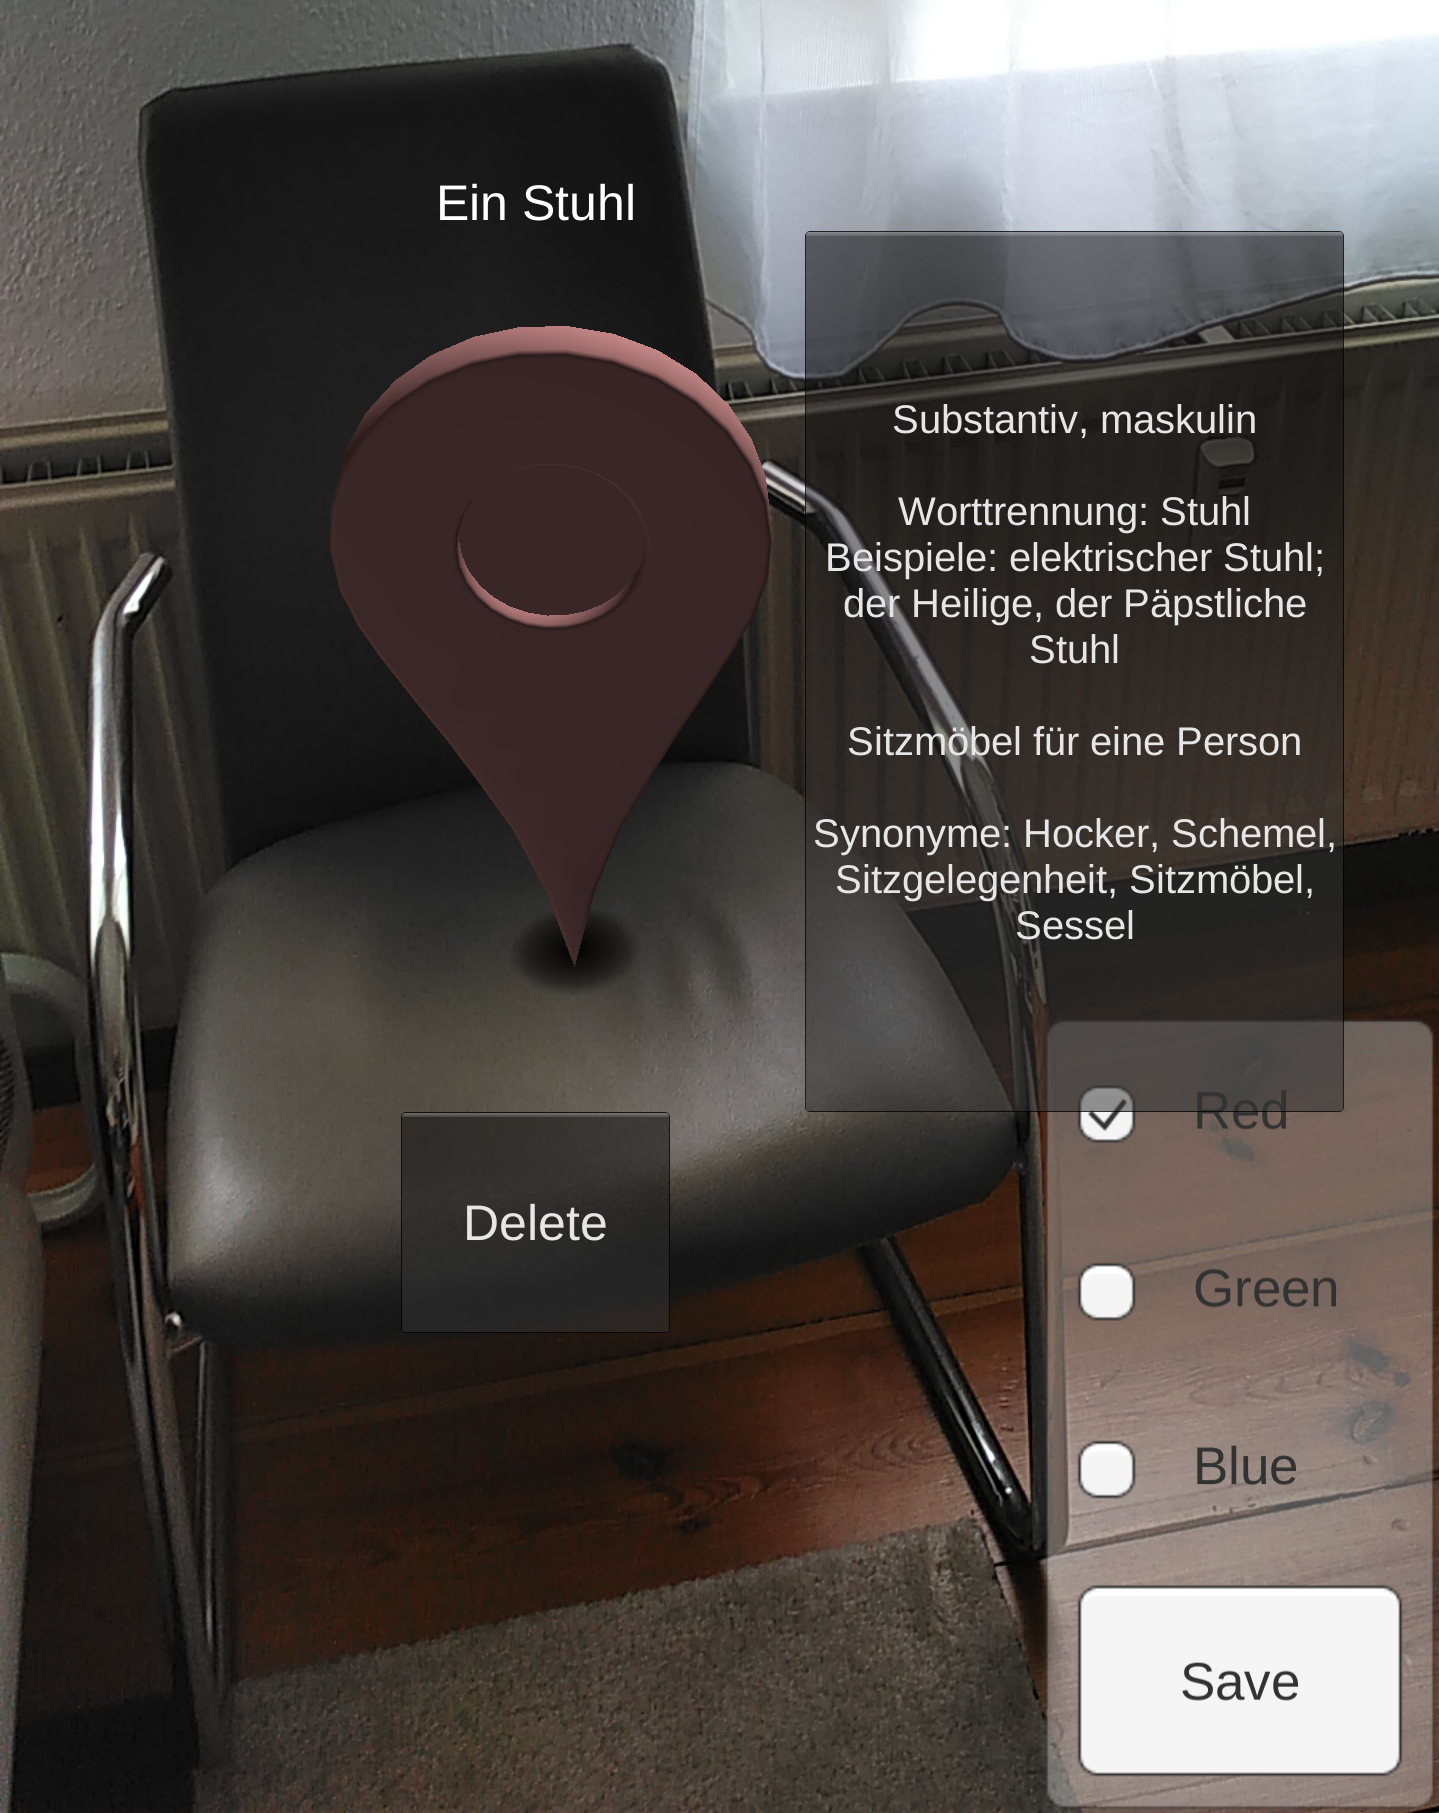
\includegraphics[width=3in]{pictures/chair}
	\caption{}
	\label{example_app_tango_unity}
\end{figure}
Neben Unity unterstützt Tango auch Java und C. Da Unity eine Game Engine ist und daher auf einer relative hohen Abstraktionsebene arbeitet, schaute ich auch in die Java API hinein. Zu dieser werden von Google keine Tutorials geliefert, jedoch haben sie auf Github eine Reihe von Beispiel-Applikationen, sowohl für Java (J)  \cite{tango_java_github} als auch für Unity (U) \cite{tango_unity_github}:

\begin{itemize}
	\item\textbf{Hello Area Description / Area Description Management (J, U):} Erstellen von Speichern von ADFs. Die App zeigt zusätzlich wann man im ADF lokalisiert ist und wann nicht.
	\item\textbf{(Simple) Augmented Reality (J, U):} Platziert Mond und Erde an die nächst beste Position. Diese gibt es einmal als reine OpenGL ES Applikation und einmal mit der Rajawali Engine.
	\item\textbf{Find Floor (U):} Sucht in der aktuell gesehen Szene die niedrigste Ebene des Raumes (Boden).
	\item\textbf{Floor Planner (J):} Erstellt den Grundriss des gescannten Gebiets.
	\item\textbf{Green Screen (J):} Simuliert einen Greenscreen mithilfe der Tiefendaten (hintere Bereiche werden ausgeblendet).
	\item\textbf{Mesh Builder (J, U):} Gleiche Funktionsweise wie der Raumscan in Unity.
	\item\textbf{Model Correspondance (J):} Platziert ein Haus zwischen vier vom Nutzer gesetzten Punkten. Die größe des Hause hängt von der mit den Punkten markierten Fläche ab.
	\item\textbf{Motion Tracking (J, U)} Zeigt eine virtuelle Welt, in der man sich über Motion Tracking bewegen kann.
	\item\textbf{Occlusion (J):} Per Tap auf dem Bildschirm wird eine Erde platziert, welche von anderen realen Objekten verdeckt werden kann.
	\item\textbf{Point Cloud (J, U):} Visualisiert die Punktwolke. Der Nutzer kann zwischen verschiedenen Perspektiven wählen. Dabei handelt es sich um eine komplexere Variante als die von den Unity-"`HowTos"'.
	\item\textbf{Point To Point (J, U):} Der Nutzer setzt zwei Punkte per Tap auf dem Bildschirm. Die Strecke zwischen den beiden Punkten wird visualisiert und die Länge wird berechnet.
\end{itemize}

Mit dem Floor Planner, der Model Correspondance App und dem Occlusion-Beispiel bieten die Java-Beispiele Funktionalitäten, die man in den Unity-Beispielen nicht findet. Dies heißt natürlich nicht automatisch, dass diese nicht in Unity umsetzbar wären. Was das Area Learning anging, war Unity jedoch die Grundlage mit dem geringeren Aufwand. Aufgrund der verschiedenen Programmiersprachen bzw. "`Entwicklungswelten"' unterscheidet sich die Entwicklung deutlich. Beim Erhalten der Daten und deren Verarbeitung sind jedoch Gemeinsamkeiten zu erkennen.